\documentclass[12pt]{article}

% a template that a friend gave, it's worked well enough for me
% i have added some packages and stuff that have proved useful

\usepackage{fancyhdr}
\usepackage{tipa}
\usepackage{fontspec}
\usepackage{amsfonts}
\usepackage{enumitem}
\usepackage[margin=1in]{geometry}
\usepackage{graphicx}
\usepackage{float}
\usepackage{amsmath}
\usepackage{braket}
\usepackage{amssymb}
\usepackage{booktabs}
\usepackage{hyperref}
\usepackage{mathtools}
\usepackage{xcolor}
\usepackage{float}
\usepackage{algpseudocodex}
\usepackage{titlesec}
\usepackage{bbm}

\pagestyle{fancy}
\fancyhf{} % sets both header and footer to nothing
\lhead{Kevin Sheng}
\setmainfont{Comic Neue}
\renewcommand{\headrulewidth}{1pt}
\setlength{\headheight}{0.75in}
\setlength{\oddsidemargin}{0in}
\setlength{\evensidemargin}{0in}
\setlength{\voffset}{-.5in}
\setlength{\headsep}{10pt}
\setlength{\textwidth}{6.5in}
\setlength{\headwidth}{6.5in}
\setlength{\textheight}{8in}
\renewcommand{\headrulewidth}{0.5pt}
\renewcommand{\footrulewidth}{0.3pt}
\setlength{\textwidth}{6.5in}
\usepackage{setspace}
\usepackage{multicol}
\usepackage{float}
\setlength{\columnsep}{1cm}
\setlength\parindent{24pt}
\usepackage [english]{babel}
\usepackage [autostyle, english = american]{csquotes}
\MakeOuterQuote{"}

\setlength{\parskip}{6pt}
\setlength{\parindent}{0pt}

\titlespacing\section{0pt}{12pt plus 4pt minus 2pt}{0pt plus 2pt minus 2pt}
\titlespacing\subsection{0pt}{12pt plus 4pt minus 2pt}{0pt plus 2pt minus 2pt}
\titlespacing\subsubsection{0pt}{12pt plus 4pt minus 2pt}{0pt plus 2pt minus 2pt}

\hypersetup{colorlinks=true, urlcolor=blue}

\newcommand{\correction}[1]{\textcolor{red}{#1}}


\begin{document}
\begin{enumerate}
    \item We're given that \[y(0)=\frac{4}{17}\cos(0)+\frac{1}{17}\sin(0)+Ce^{0}=-1\]
          Solving the equation for $C$: \begin{gather*}
              \frac{4}{17} \cdot 1 +\frac{1}{17} \cdot 0+C \cdot 1=-1 \\
              C=-\frac{21}{17}
          \end{gather*}
          Thus, given the initial conditions, we have \[\boxed{y(t)=\frac{4}{17}\cos(t)+\frac{1}{17}\sin(t)-\frac{21}{17}e^{-4t}}\]
          \begin{center}
              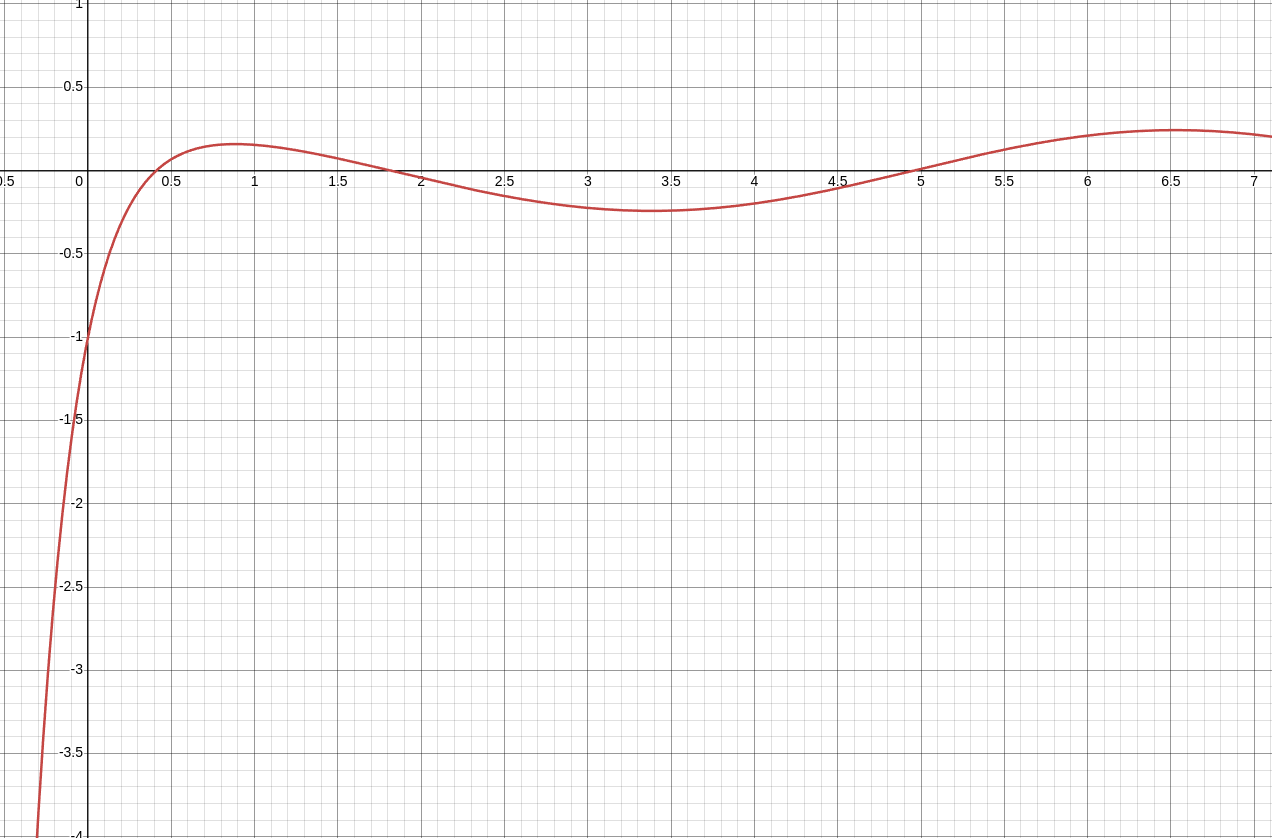
\includegraphics[width=8cm]{img/graph1} \\
              \small{A snapshot of this equation centered around $x=6$.}
          \end{center}
    \item As in the previous question, plug in the initial conditions and solve for $C$ first:
          \begin{gather*}
              y(1)=e^{-1}(1+\frac{C}{1})=\frac{1}{e} \\
              1+C=1 \\
              C=0 \\
              \boxed{y(t)=e^{-t} \cdot t}
          \end{gather*}
          \begin{center}
              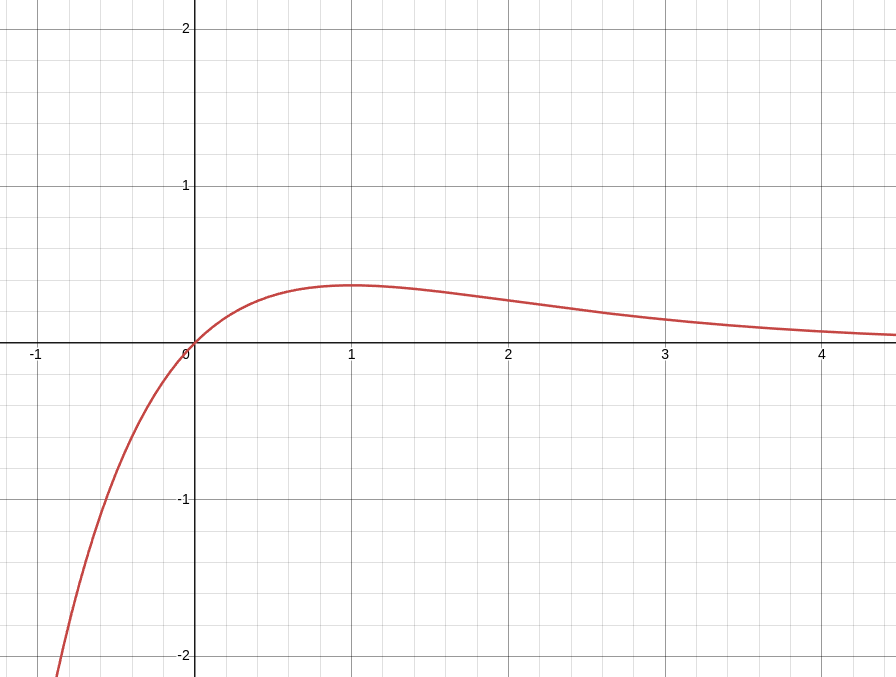
\includegraphics[height=4cm]{img/graph2} \\
          \end{center}

          \pagebreak

    \item This is a separable equation, so we can isolate the variables and integrate.
          \begin{align*}
              \frac{dy}{dx} & =\frac{xy}{x-1}       \\
              \frac{dy}{y}  & =\frac{x\,dx}{x-1}    \\
              \ln |y|       & =x+\ln |x-1|+C        \\
              |y|           & =\exp(x+\ln |x-1|+C)  \\
              \Aboxed{y     & = \pm e^C \cdot e^x |x-1|}
          \end{align*}
    \item
          \begin{align*}
              \frac{dy}{1+y^2} & =dx        &  & \text{Isolate $x$ and $y$}  \\
              \arctan(y)       & =x+C       &  & \text{Integrate both sides} \\
              y                & =\tan(x+C)
          \end{align*}
          For $y(0)=1$, we need $\tan(x+C)=1$ which means that $C=\frac{\pi}{4}$ and $\boxed{y=\tan\left(x+\frac{\pi}{4}\right)}$.
          Since $\tan(x)$ is undefined at $x=\pm\frac{\pi}{2}$, our interval of existence is $\boxed{x \in \left(-\frac{3\pi}{4}, \frac{\pi}{4}\right)}$.
    \item First, manually check if the edge cases $y=x^0$ and $y=x^1$ work.
          \begin{gather*}
              x^2 \cdot 0 - 3x \cdot 0-32 \cdot 1 \ne 0\text{ so } y=x^0\text{ doesn't work}\\
              x^2 \cdot 0 - 3x \cdot 1 - 32 \cdot x \ne 0\text{ so }y=x^1\text{ isn't good either}\\
          \end{gather*} With those out of the way, if $y=x^n$, then and $y'=nx^{n-1}$ and $y''=n(n-1)x^{n-2}$
          \begin{align*}
              n(n-1)x^n-3nx^n-32x^n & =0 \\
              n(n-1)-3n-32          & =0
          \end{align*}
          Factoring and solving this quadratic equation yields $\boxed{n=-4\text{ or }8}$.
    \item I'll assume $t$ is measured in hours since the time of the discovery of the body.
          \begin{align*}
              \frac{dT}{dt}   & =k(50-T)     \\
              \frac{dT}{50-T} & =k\,dt       \\
              -\ln |50-T|     & =kt+C        \\
              |50-T|          & =e^{-kt+C}   \\
              50-T            & =Ce^{-kt}    \\
              T               & =50-Ce^{-kt}
          \end{align*}
          Since $T(0)=70$, $C=-20$, and now we solve for $k$:
          \begin{align*}
              60          & =50+20e^{-2k}                             \\
              \frac{1}{2} & =e^{-2k}                                  \\
              k           & =\frac{\ln \frac{1}{2}}{-2}\approx 0.3466
          \end{align*}
          With this, we can finally solve for the time when $T=98.6$:
          \begin{align*}
              98.6                & = 50+20e^{-kt}                                        \\
              \frac{48.6}{20}     & = e^{-kt}                                             \\
              \ln \frac{48.6}{20} & = -kt                                                 \\
              t                   & =\frac{\ln \frac{48.6}{20}}{-k} \approx \boxed{-2.56}
          \end{align*}
          The murder took place around 5:30 PM\@.
\end{enumerate}
\end{document}